\clearpage
\section{Discriminators and tagging rates \label{sec:discriminators}}
Details about the calculation of the discriminators are given in~\cite{btaggingPAS2009}. The distributions of track counting discriminators are shown in Figure~\ref{fig:trackCountingDisc}, jet probability discriminators are shown in Figure~\ref{fig:JetProbDisc} and simple secondary vertex discriminators are shown in Figure~\ref{fig:SimpleSVDisc}. 

\begin{figure}[h!]
\centering
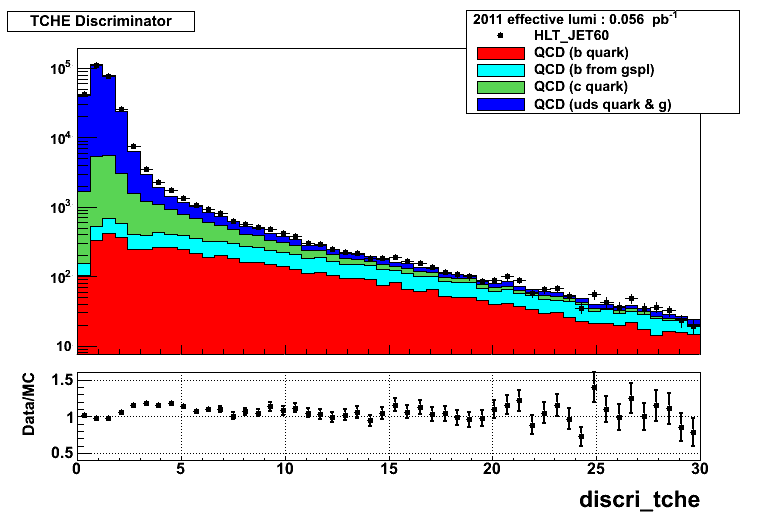
\includegraphics[width=0.45\textwidth]{figures/discri_tche_Log.png}
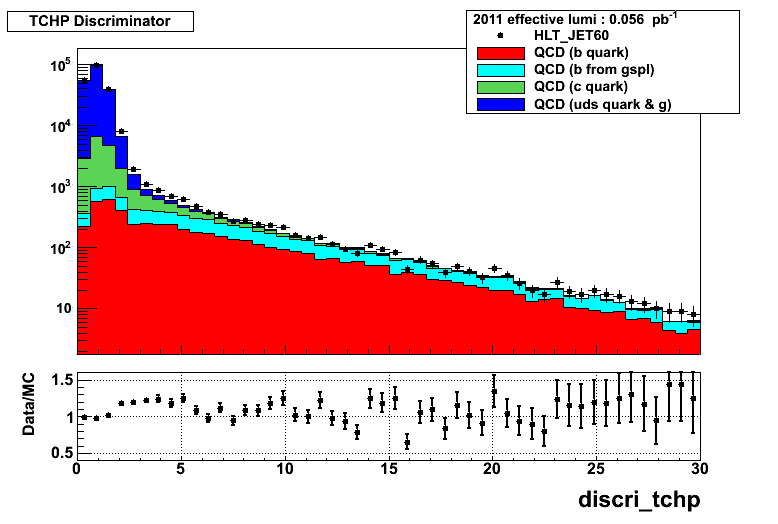
\includegraphics[width=0.45\textwidth]{figures/discri_tchp_Log.png}
\caption{Left: track counting high efficiency, Right: track counting high purity discriminators. }
\label{fig:trackCountingDisc}
\end{figure}
\begin{figure}[h!]
\centering
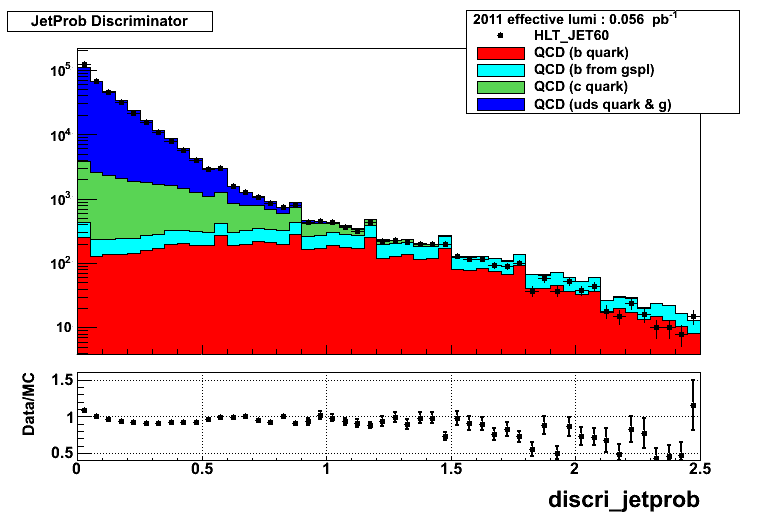
\includegraphics[width=0.45\textwidth]{figures/discri_jetprob_Log.png}
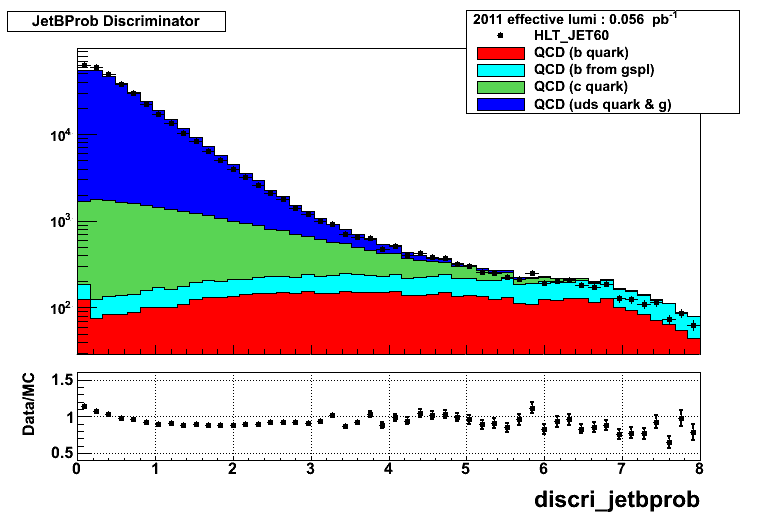
\includegraphics[width=0.45\textwidth]{figures/discri_jetbprob_Log.png}
\caption{Left: jet probability , Right: jet B probability discriminators. }
\label{fig:JetProbDisc}
\end{figure}
\begin{figure}[h!]
\centering
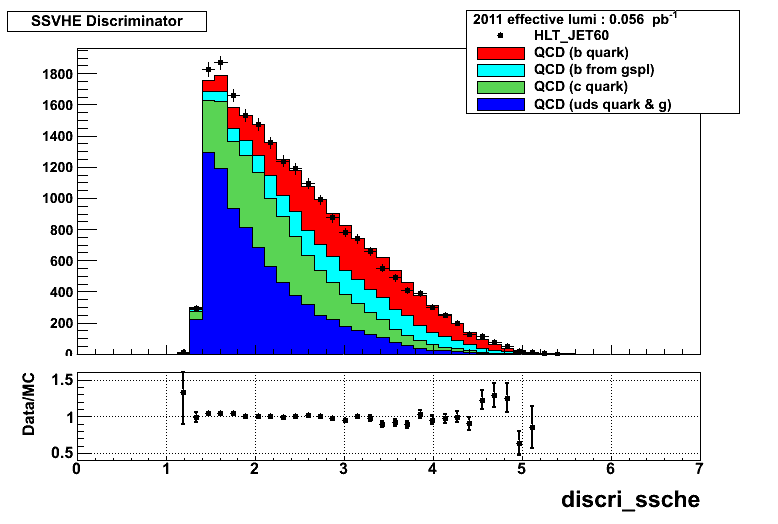
\includegraphics[width=0.45\textwidth]{figures/discri_ssche_Linear.png}
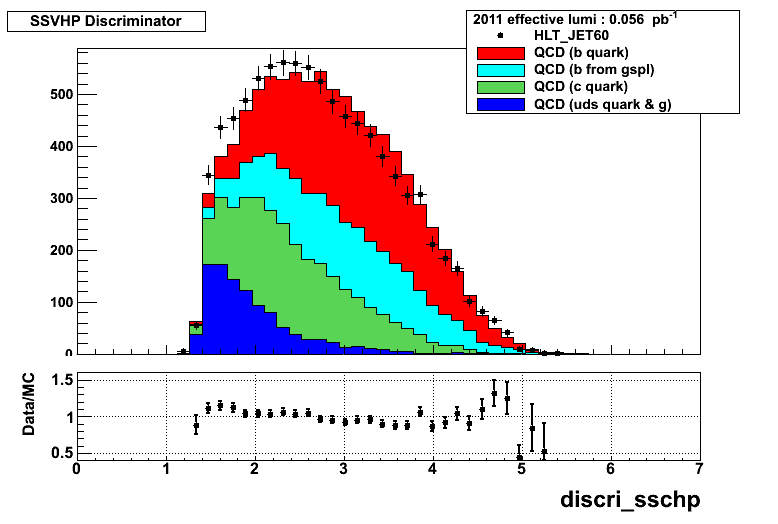
\includegraphics[width=0.45\textwidth]{figures/discri_sschp_Linear.png}
\caption{Left: simple secondary vertex high efficiency , Right: simple secondary vertex high purity discriminators. The underflow bin for jets which do not contain a reconstructed secondary vertex is not displayed.}
\label{fig:SimpleSVDisc}
\end{figure}

The tagging rates can be calculated by integrating the discriminator distributions (Figures \ref{fig:trackCountingDisc} to \ref{fig:SimpleSVDisc}) from a given discriminator cut to infinity, divided by the total integral.  The tagging rates are displayed in Figures~\ref{fig:trackCountingDiscEff} to \ref{fig:SimpleSVDiscEff}.

\begin{figure}[h!]
\centering
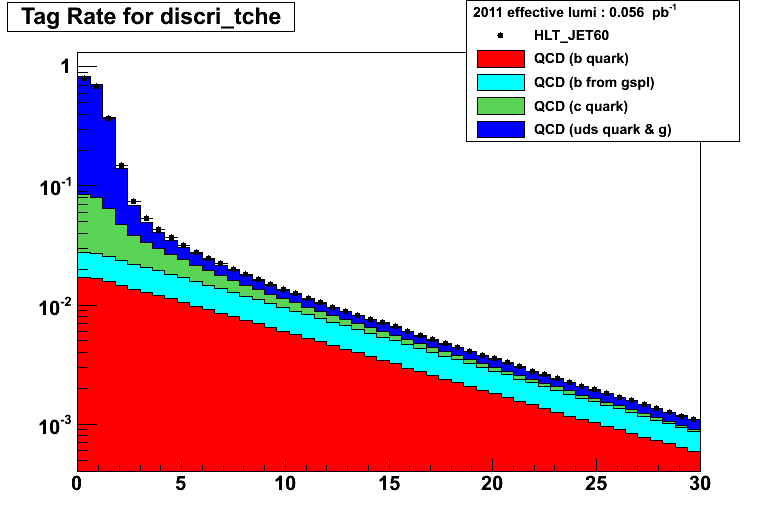
\includegraphics[width=0.45\textwidth]{figures/tagRate_discri_tche_Log.png}
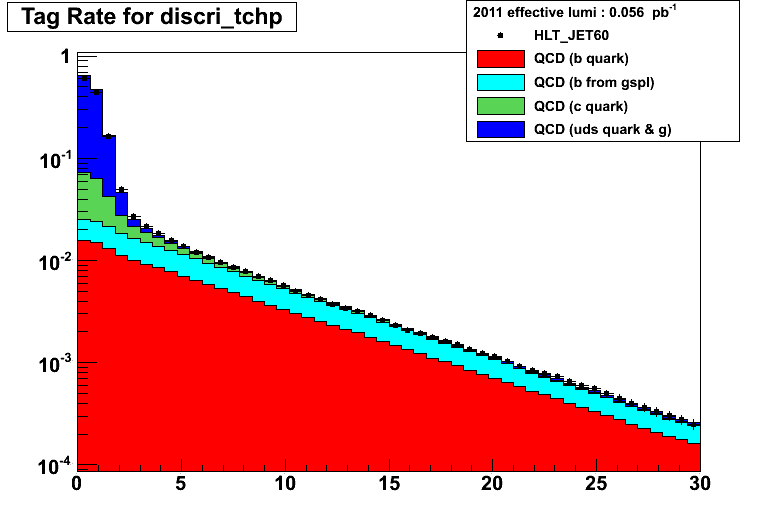
\includegraphics[width=0.45\textwidth]{figures/tagRate_discri_tchp_Log.png}
\caption{Left: track counting high efficiency tagging rate, Right: track counting high purity tagging rate. }
\label{fig:trackCountingDiscEff}
\end{figure}
\begin{figure}[h!]
\centering
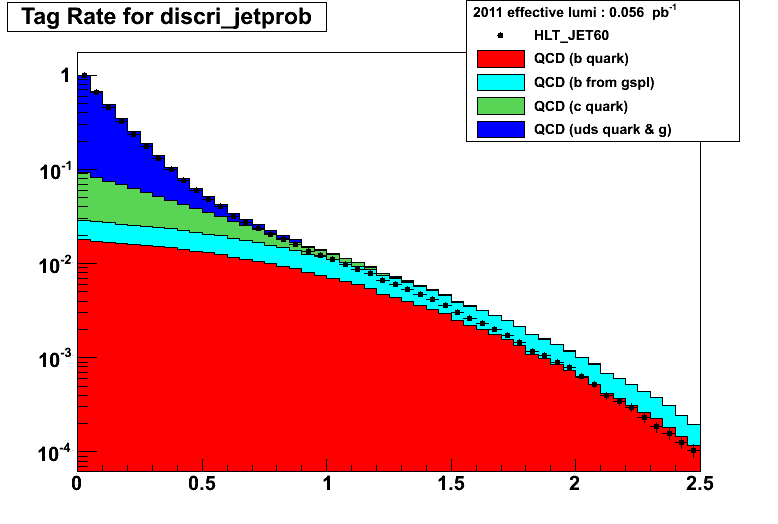
\includegraphics[width=0.45\textwidth]{figures/tagRate_discri_jetprob_Log.png}
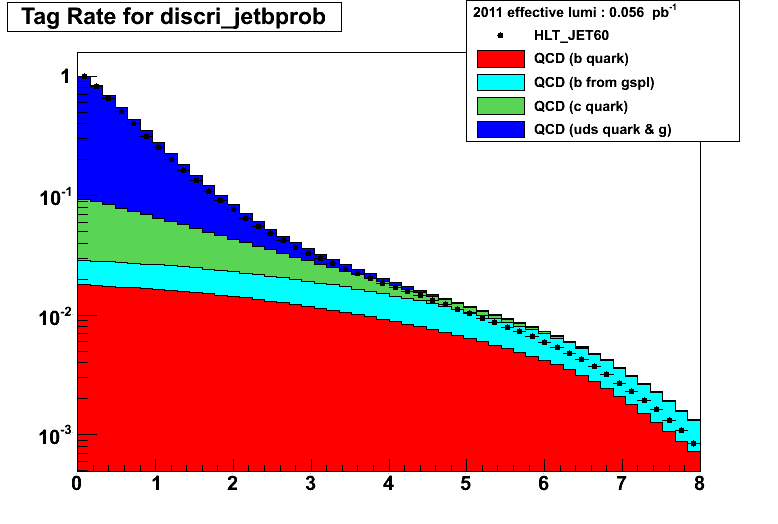
\includegraphics[width=0.45\textwidth]{figures/tagRate_discri_jetbprob_Log.png}
\caption{Left: jet probability tagging rate, Right: jet B probability tagging rate. }
\label{fig:JetProbDiscEff}
\end{figure}
\begin{figure}[h!]
\centering
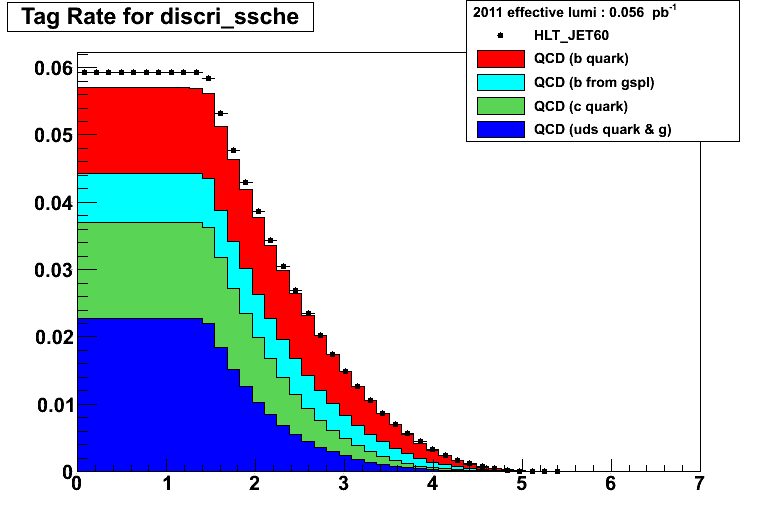
\includegraphics[width=0.45\textwidth]{figures/tagRate_discri_ssche_Linear.png}
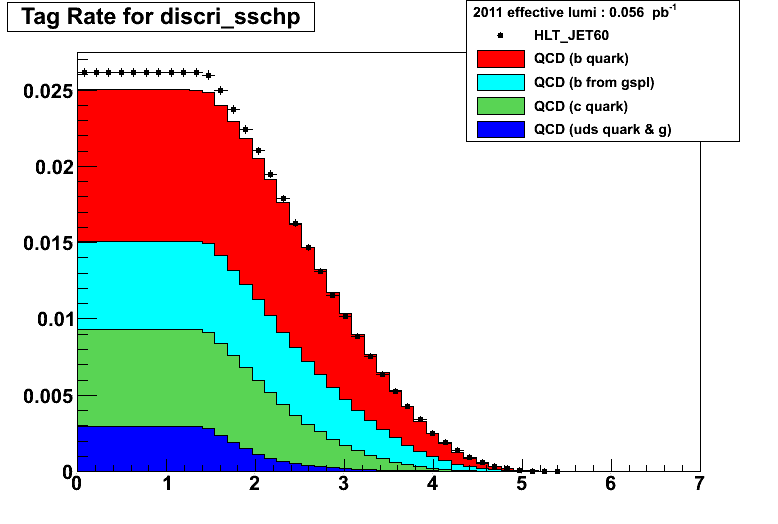
\includegraphics[width=0.45\textwidth]{figures/tagRate_discri_sschp_Linear.png}
\caption{Left: simple secondary vertex high efficiency tagging rate, Right: simple secondary vertex high purity tagging rate. }
\label{fig:SimpleSVDiscEff}
\end{figure}